\chapter{Latome Hardware Design}\label{ch:latome-firmware}
% \parskip4pt \parindent12pt

\section{Specifications}\label{sec:specifications}
\subsection{The Liquid Argon Calorimeter Data Path}\label{sec:lar}
The LAr Calorimeter is made of approximately 180,000 cells measuring energies which are summed up in the digital trigger path to form 34,048 artificial Super Cells. This summing is necessary to reduce the amount of data being processed at the cost of a lower granularity. The 12-bit readings of 8 Super Cells are serialized into one packet and sent through one optic fiber. The 116 LATOME boards are each connected to 48 optic fibers, thus receiving data from up to \(48\times8=384\) Super Cells. These boards take care of:

\begin{itemize}
    \item Deserializing the input data
    \item Aligning them into a single clock domain for combined data processing
    \item Computing the estimated energy value
    \item Identifying the Bunch Crossing ID of a respective pulse
    \item Encoding the output data
    \item Serializing and transmitting the data to different Feature Extractors (FEX) systems
\end{itemize}

The FEX system processes the data and sends it to the Level 1 Trigger system. It contains 3 groups: the Global Feature Extractor (gFEX), the Jet Feature Extractor (jFEX) and the Electron Feature Extractor (eFEX). Within these groups, gFEX uses one board which gets summed data from all LATOMEs, thus showing the lowest granularity but with one board covering the whole detector. Then the jFEX uses 6 boards, each receiving data from up to 19 LATOMEs, and finally the eFEX, with the highest granularity, uses 24 boards, each receiving data from up to 4 LATOMEs.

\subsection{The LATOME Specifications}\label{sec:latome-specifications}
The part of the LATOME firmware which converts ADC levels into energy levels is called \textit{User Code} in the LAr group. The LATOME HLS team does not own this code. However, the team develops the blocks for the different data organization steps, also called mapping or remapping, and the summing of energies for LATOMEs in specific regions of the detector. Additionally, since the output energies are only encoded on 10 bits for the eFEX and 12 bits for the jFEX and gFEX, it is necessary to compress the data from 12 to 10 bits for the former or 22 to 12 bits for the latter via a Multi Linear Encoder (MLE).

Initially, a Russian team developed the whole LATOME firmware in VHDL. The implementation of all the functionalities took over 8 years and still had timing violations. 

Timing violations are a common issue in FPGA designs. They happen when the design is not able to meet the timing constraints set by the user. For instance, the setup time of a flip-flop is the time required for the input to be stable before the clock edge, and the hold time is the time required for the input to be stable after the clock edge. If the input is not stable during these times, the flip-flop can go into a metastable state, which can lead to unpredictable behavior.

Because in the next runs of the LHC, the amount of energy and luminosity is expected to increase, the LATOME design should be optimized to leave space for other functionalities and more complex algorithms to keep high trigger efficiency.

\section{Current LATOME Firmware}\label{sec:existing-design}

% The original design is characterized by more clock domain crossings than the current one.

\begin{figure}
    \centering
    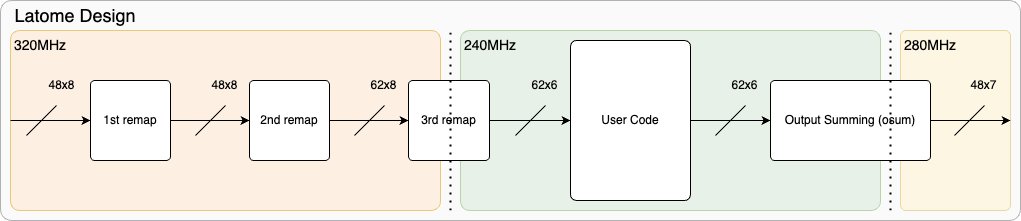
\includegraphics[width=1\textwidth]{latome_fw_vhdl.png}
    \caption{Original VHDL Design}
    \label{fig:original-vhdl-design}
\end{figure}

Because bunch crossings (BC) happen at a frequency of 40MHz, it is necessary to run the different blocks of the design at multiples of this frequency. The Figure \ref{fig:original-vhdl-design} shows three different frequencies being used. At the first remap stage, since the frames are made of 8 words, it is necessary to run the blocks at 320MHz. Then the frames become 6 words long, corresponding to a frequency of 240MHz. Finally, the FEX systems expect 7 32 bits words, thus the frequency is 280MHz.

\begin{figure}[htb]
    \centering
    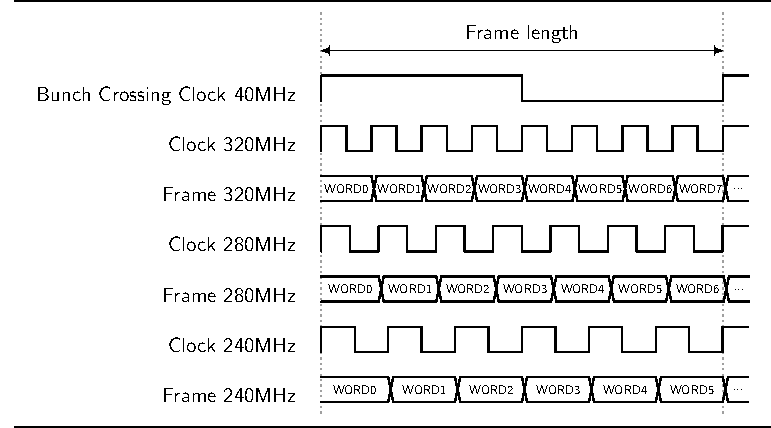
\includegraphics{timings/bc_clocks}
    \caption{Different clocks used in the design}
    \label{fig:bc-clocks}
\end{figure}

These clock domain crossings made the original implementation very complex...
%TODO: add more about the complexity of the original design

\section{Leveraging Time vs Space Division Multiplexing}\label{sec:leveraging-time-division-multiplexing}

When a chunk of data is available at a given time for processing, it can all be processed at the same time, or pieces after pieces.
Processing simultaneously all the data offers the advantage of a reduced latency, but requires creating copies of the processing blocks for each piece. A sequential processing gives the possibility of having just one block processing portions of the data each clock cycle at the price of latency.

\subsection{Time Division Multiplexing}\label{sec:time-division-multiplexing}
The time division multiplexing approach consists in sharing the resources, or processing blocks, by routing each piece of data depending on time \(t\). Choosing this implementation can be intuitive as computers usually process data using frames of 32 to 64 bits. It has the advantage of reusing design blocks hence possibly reducing area usage, but performs poorly in case of data dependencies. If the word from time \(t=0\) of the frame needs to be available at the same time as the one of \(t=4\), the logic becomes very complex thus canceling the positive area impact unlocked by resource sharing in some cases.

The part (a) of Figure \ref{fig:time-division-multiplexing} shows a block diagram representing the logic needed to reuse a given block using TDM. The multiplexer on the left routes the data from the five input registers, \verb|input0| to \verb|input4|, to an intermediate \verb|input| register, at 5 predefined time slots, in a periodic manner. A given input of the register will be connected again to the output of the multiplexer after 5 clock cycles. The intermediate \verb|input| register is only used for the Timing analysis in part (b) of the figure. A counter with module 5 drives the selection input of the multiplexer. The grey square box represents the processing block which is reused at each time slot. The multiplexer on the right implements the inverse functionality of the first one, routing the output of the processing block, \verb|output|, to the output registers, \verb|output0| to \verb|output4|. The timing diagram in part (b) shows the different signals of the block diagram. The \verb|input0| and \verb|input1| are constant for 5 clock cycles, while the output of the first multiplexer, \verb|input|, changes every clock cycle. Considering a latency of 2 clock cycles, the timing shows that the \verb|output0| receives the output of the processing block after 2 clock cycles. The \verb|output1| receives the output of the processing block after $2+1=3$ clock cycles, and so on. 

\begin{figure}
    \begin{subfigure}[c]{.5\textwidth}
        \centering
        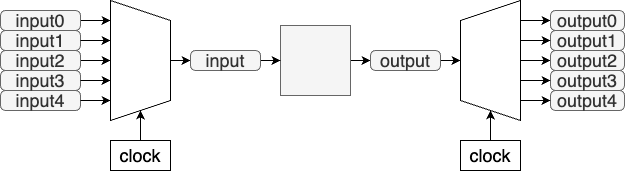
\includegraphics[width=1\linewidth]{tdm.png}
        \caption{Block Diagram}
    \end{subfigure}
    \begin{subfigure}[c]{.5\textwidth}
        \centering
        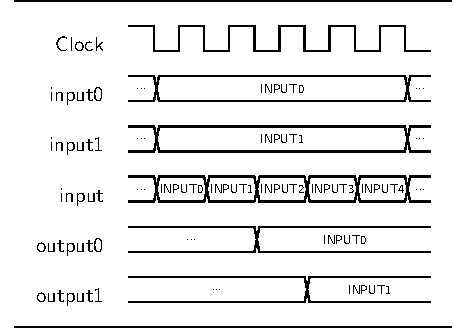
\includegraphics[width=1\linewidth]{../timings/tdm.pdf}
        \caption{Timing}
    \end{subfigure}
    \caption{Time Division Multiplexing}
    \label{fig:time-division-multiplexing}
\end{figure}

\subsection{Space Division Multiplexing}
Another way of processing the data is to make it all available at the same time, as parallel inputs of the processing block. This approach is more natural as it is closer to what humans experience; we see, hear, feel, taste at the same time, not one after the other. 

Similarly to what is shown in Figure in Figure \ref{fig:time-division-multiplexing}, Figure \ref{fig:space-division-multiplexing} presents a SDM block diagram and timing. The block diagram in part (a) shows 5 input registers, \verb|input0| to \verb|input4|, all connected to their own copy of the processing block, represented by the 5 grey rectangles. The output of the processing block is directly connected to the output registers, \verb|output0| to \verb|output4|. Part (b) of the figure shows the signals from the registers \verb|output0| and \verb|output1| receiving the output of the processing block simultaneously after 2 clock cycles.

Space Division Multiplexing generally offers lower latencies, as every block runs in parallel and reduces the use of sequential logic which would be required in TDM. In fact, using a parallel logic, some processing blocks can become purely combinational ones.

\begin{figure}
    \begin{subfigure}{.5\textwidth}
        \centering
        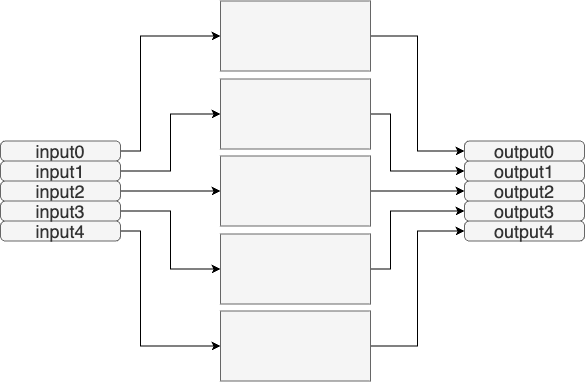
\includegraphics[width=1\linewidth]{sdm.png}
        \caption{Block Diagram}
    \end{subfigure}
    \begin{subfigure}{.5\textwidth}
        \centering
        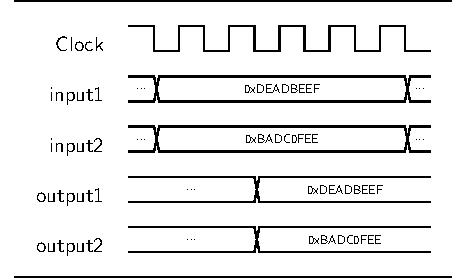
\includegraphics[width=1\linewidth]{../timings/sdm.pdf}
        \caption{Timing}
    \end{subfigure}
    \caption{Space Division Multiplexing}
    \label{fig:space-division-multiplexing}
\end{figure}

\subsection{Tradeoffs}\label{sec:space-versus-time-division-multiplexing}
Whether one approach is better than the other is difficult to determine prior to having a deep understanding of the data processing blocks. The most common tradeoff is the one of latency at the price of area. But the Maximal Operating Frequency (\(F_{max}\)) can also be traded to improve other metrics.

Having access to all variables at the same time, in the case of SDM makes the code development easier. For example, to implement a sorting algorithm, it is easier to sort all the data when it is all available at the same time, than to sort it piece by piece.

\section{New HLS Design}\label{sec:current-hls-design}
When developing the new firmware from the specifications in HLS, very interesting insights from Dr. Marcos Oliveira emphasizing benefits of space division multiplexing were taken into account. With a parallel implementation, the logic is significantly simplified and does not depend anymore on the frame length. It also allows retargeting the circuit to different clock frequencies, because it is no longer limited by the serial interfaces.

\begin{figure}
    \centering
    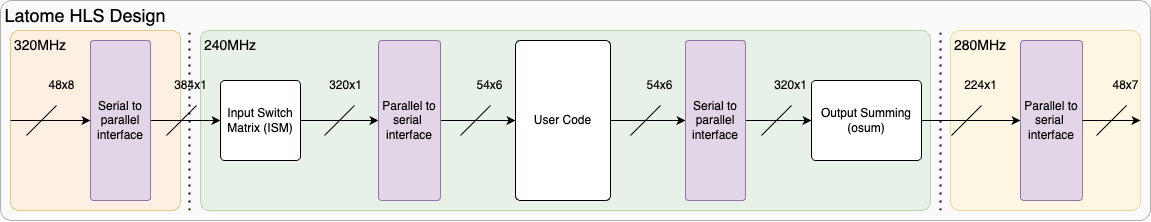
\includegraphics[width=1\textwidth]{latome_fw_hls.png}
    \caption{Current HLS Design}
    \label{fig:current-HLS-design}
\end{figure}

The figure \ref{fig:current-HLS-design} shows that all the remapping and processing blocks except for the User Code are processing data in parallel. This is possible thanks to the serial-to-parallel and parallel-to-serial data transformation blocks. This approach drastically simplifies the design and showed very promising results in terms of area reduction, reduced latency.
% TODO: add more promising results

\begin{figure}
    \centering
    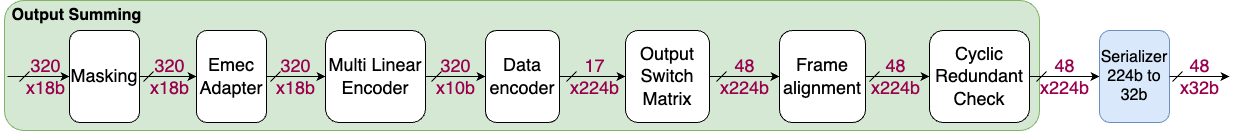
\includegraphics[width=1\textwidth]{osum_v6.png}
    \caption{Output Summing Block Diagram}
    \label{fig:osum-v6}
\end{figure}

The Output Summing was completely redesigned and broken down in different blocks which are represented in figure \ref{fig:osum-v6}. It includes the following blocks:
\begin{itemize}
    \item Masking: responsible for disabling some inputs to suppress noisy Super Cells.
    \item Emec Adapter: this block distributes the original energy from 11 to 9 Super Cells in the EMEC region of the detector to fit within the maximum number of 10 Super Cells per trigger tower.
    \item Multi Linear Encoder (MLE): Performs data compression by mapping 18 to 22-bit energy value to 10 to 12-bit encoded values using a pre-defined multi-linear encoding table.
    \item Data Encoder: Packs the encoded energy value and timing information into 17 224-bit frames using a predefined data format.
    \item Output Switch Matrix (OSM): This switch matrix routes the 17 224 bits frames to each of the FEX system modules connected to the respective LATOME.
    \item Frame Alignment: One BC per orbit, the LATOME does not send any data but instead it sends an alignment frame built by this block.
    \item CRC9: This final block appends to the last 9 bits of each frame the computed CRC-9 value of the transmitted data that is later used at the FEX system to check the received data against errors.
\end{itemize}